\documentclass[../main-notes.tex]{subfile}

\begin{document}

\section{Recap}

\subsection{Parabola}

\begin{marginfigure}
    \centering
    \includegraphics[width=\textwidth]{../Figures/parabola/ParabolaDirectrix_1002.png}
    \caption{Parabola}\label{fig-parabola-recap}
\end{marginfigure}


\begin{gather*}
    \sqrt{(x-a)^2 + y^2} = x+a\to\qty(y-k)^2 = 4a\qty(x-h) \\
    \sqrt{x^2 + (y-a)^2} = y+a\to\qty(x-h)^2 = 4a\qty(y-k)
\end{gather*}

\begin{note}{Expanded form}{~}
 \begin{align*}
    \qty(x-h)^2 &= 4a\qty(y-k) \\
    x^2 -2hx +h^2 &= 4ay-4ak \\
    \frac{1}{4a}\qty[4ay] &=\frac{1}{4a}\qty[x^2 -2hx + h^2 +4ak] \\
    y &=\frac{x^2}{4a} -\frac{hx}{2a} +\frac{h^2}{4a}  +k 
\end{align*}

In this case this function (a parabola with horizontal directrix) is bijective and has the following domain and range $x\in(-\infty,\infty)$ and $f(x,y)\in\qty(-\infty,\infty)$.
However, we need to be careful, because the parabola with a vertical directrix is not a bijective function, because for each value of $x$ it corresponds two values of $y$.
   
\end{note}



\subsection{Circle}

\begin{marginfigure}
    \centering
    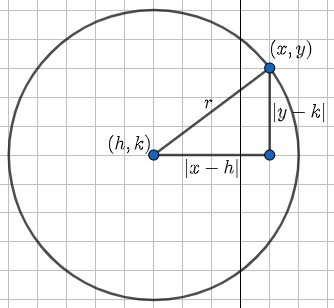
\includegraphics[width=\textwidth]{../Figures/circunference/circle-translate.jpg}
    \caption{Circle}\label{fig-circle-recap}
\end{marginfigure}

\begin{gather}
    a^2 + b^2 = c^2\to\qty(x-h)^2 + \qty(y-k)^2 = r^2
\end{gather}

\begin{note}{Expanded form}{note-jiji}
    We are going to expand the equation\eqref{eqn:circle-displaced} to get familiarize ourselves with different expressions of the same mathematical object.
    \begin{align*}
        \qty(x-h)^2 + \qty(y-k)^2 &= r^2 \\
        \qty(x^2 -2hx + h^2) + \qty(y^2 -2ky + k^2) &= r^2 \\
        x^2 + y^2 -2hx -2ky + h^2 + k^2 &= r^2
    \end{align*}

    As we can see, this can be approach as a function of two independent variables $x$ and $y$ ($f(x,y)$) equated to a constant value $r^2$, $f(x,y)=r^2$.
    This function is not bijective, indicating that there is no inverse function and the domain and range are bounded.

\end{note}


\subsection{Ellipse}

\begin{marginfigure}
    \centering
    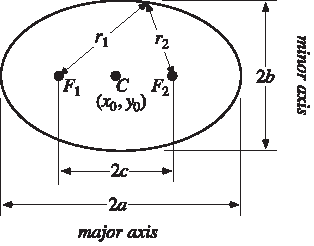
\includegraphics[width=\textwidth]{../Figures/ellipse/EllipseBipolar_700.pdf}
    \caption{Ellipse}\label{fig-ellipse-recap}
\end{marginfigure}

\begin{align*}
    \sqrt{(x-c)^2+y^2} + \sqrt{(x+c)^2+y^2} = 2a\to\frac{\qty(x-h)^2}{a^2} + \frac{\qty(y-k)^2}{b^2} &= 1.
\end{align*}

\begin{note}{Expanded form}{~}
Now we are going to expand the expression,
\begin{align*}
    \frac{\qty(x-h)^2}{a^2} + \frac{\qty(y-k)^2}{b^2} &= 1 \\
    \frac{1}{a^2}\qty(x^2-2xh+h^2) + \frac{1}{b^2}\qty(y^2-2yk+k^2) &= 1 \\
    \frac{x^2}{a^2} + \frac{y^2}{b^2}
    -\frac{2xh}{a^2} -\frac{2yk}{b^2}
    +\frac{h^2}{a^2} + \frac{k^2}{b^2} &= 1
\end{align*}

As same with the circle equation, we can approch this as a two variable function $f(x,y)$ equated to $1$, $f(x,y)=1$.
However, we need to take into account that this is not a bijective function, which leads to have a bounded domain and range with no inverse function.
\end{note}

\subsection{Hyperbola}

\begin{marginfigure}
    \centering
    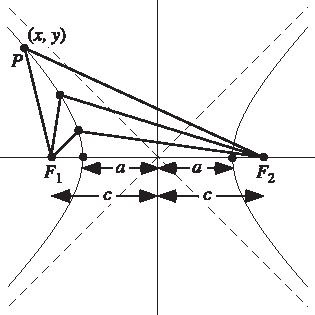
\includegraphics[width=\textwidth]{../Figures/hyperbola/HyperbolaFoci_750.pdf}
    \caption{Hyperbola}\label{fig-hyperbola-recap}
\end{marginfigure}

\begin{gather*}
    \sqrt{\qty(x-c)^2+y^2} - \sqrt{\qty(x+c)^2+y^2} = 2a\to\frac{\qty(x-h)^2}{a^2} - \frac{\qty(y-k)^2}{b^2} = 1
\end{gather*}

\begin{note}{Expanded equation}{~}
    For completeness, we are going to expand the quadratic terms,
    \begin{align*}
        \frac{\qty(x-h)^2}{a^2} - \frac{\qty(y-k)^2}{b^2} &= 1 \\
        \frac{1}{a^2}\left[x^2-2hx+h^2\right] -\frac{1}{b^2}\left[y^2-2ky+k^2\right] &= 1 \\
        \frac{x^2}{a^2}-\frac{2hx}{a^2}+\frac{h^2}{a^2}  -\frac{y^2}{b^2}+\frac{2ky}{b^2}-\frac{k^2}{b^2} &= 1
    \end{align*}

    This equation ($f(x,y)=1$) is not a bijective function.
    On the other hand, the range can go from plus infinity to minus infinity $f(x,y)\in\qty(-\infty,\infty)$, however, the domain is not defined between the distance of the two vertex $x\in(-\infty,h-a]\cup[h+a,\infty)$.
\end{note}

\begin{note}{Asymptotes of the hyperbola}{~}
    As mentioned in the note before, the domain is not defined in the inverval $x\in(h-a,h+a)$, indicating the existance of asymptotes.
    Here we are going to see the derivation of the asymptotes.
    To do that, we are going to equate the function to zero $f(x,y)=0$,
    \begin{align*}
        \frac{\qty(x-h)^2}{a^2} - \frac{\qty(y-k)^2}{b^2} = 1 &\to\frac{\qty(x-h)^2}{a^2} = \frac{\qty(y-k)^2}{b^2} \\
        \left[\qty(x-h)^2\right]^{1/2} &= \left[\frac{a^2}{b^2}\qty(y-k)^2\right]^{1/2} \\
        x-h &= \pm\frac{a}{b}\qty(y-k) 
    \end{align*}
\end{note}

\subfile{exercises.tex}

\end{document}
